\documentclass[14pt, aspectratio=169]{beamer}
\usepackage[magyar]{babel}
\usepackage[utf8]{inputenc}
\usepackage[T1]{fontenc}
\usepackage{graphicx}
\usepackage{subcaption}
\usepackage{siunitx}
\usepackage{booktabs}
\usepackage[font=footnotesize]{caption}
\captionsetup[sub]{font=footnotesize}
\captionsetup{labelformat=empty}

\graphicspath{{/home/istvan/insar/images/}}
\DeclareGraphicsExtensions{.png,.jpg}


\newcommand{\backupbegin}{
   \newcounter{finalframe}
   \setcounter{finalframe}{\value{framenumber}}
}
\newcommand{\backupend}{
   \setcounter{framenumber}{\value{finalframe}}
}

\newcommand{\stamps}{\texttt{StaMPS} }

\usetheme{Boadilla}
\usecolortheme{whale}

\title[Radar interferometria]{Felszíni deformációs sebességek becslése a Csomád vulkán térségében állandó szórópontú radarinterferometria segítségével}
\author{Bozsó István}
\date{2017.06.12.}

\begin{document}

%-----------------------------------------------------------------------------

\begin{frame}
    \begin{figure}
        \centering
        
\includegraphics[width=0.2\linewidth]{ggi_logo.png}
    \end{figure}

    \center{\bfseries Felszíni deformációs sebességek becslése a Csomád vulkán térségében állandó szórópontú radarinterferometria segítségével}

    \vspace{15pt}

    \begin{minipage}[t]{0.3\textwidth}
        {\footnotesize Bozsó István\\Geofizika MSc.}
    \end{minipage}
    \begin{minipage}[t]{0.3\textwidth}
        {\footnotesize Szűcs Eszter\\Bányai László}
    \end{minipage}
\end{frame}

%-----------------------------------------------------------------------------

\begin{frame}{Áttekintés}

    \begin{enumerate}
        \item Bevezetés - InSAR technológia, Csomád-vulkán
        \item Adatok és feldolgozásuk
        \item Eredmények
        \item Összefoglalás
    \end{enumerate}

\end{frame}

%-----------------------------------------------------------------------------

\begin{frame}{SAR technológia}
    \begin{figure}
        \centering
        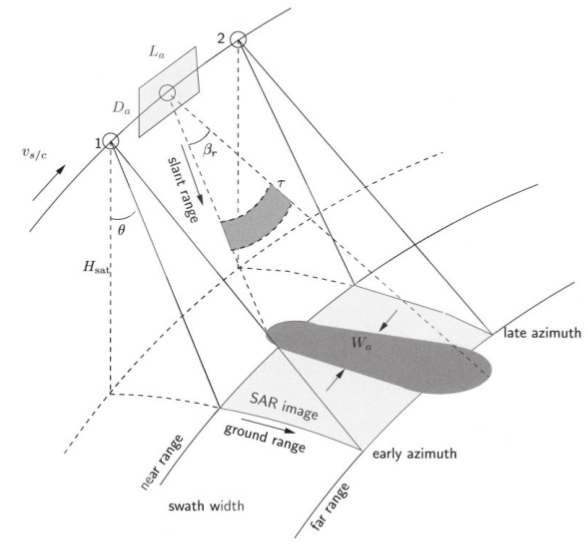
\includegraphics[height=145pt]{ramon_SAR.png}
        \caption{SAR felvétel készítésének geometriája.}
    \end{figure}
    \vspace{-35pt}
    \center{Felbontás növelése: $5-\SI{10}{\kilo\meter} \rightarrow \SI{10}{\meter}$}
\end{frame}

%-----------------------------------------------------------------------------

\begin{frame}{InSAR alapgondolat}
    \begin{figure}
        \centering
        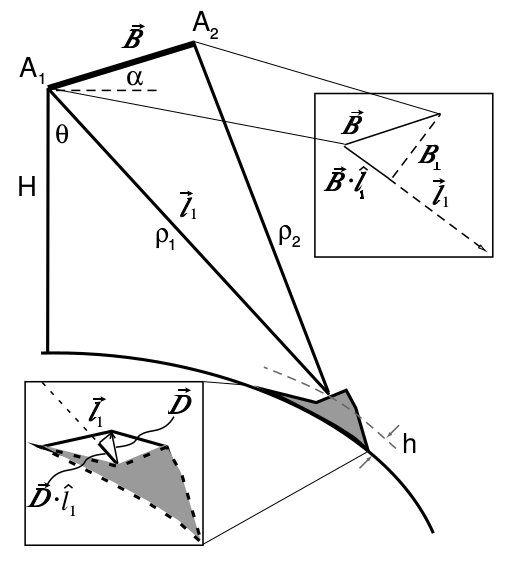
\includegraphics[height=160pt]{burgmann_geom.png}
       \caption{Két SAR felvétel készítésének geometriája. A két felvétel fáziskülönbsége több tagból adódik: a felvételi pozíciók (náhány száz méteres) eltéréséből ($\vec{B} \ne 0$) és a felszíni deformációból ($\vec{D}$)}
    \end{figure}
\end{frame}

%-----------------------------------------------------------------------------

\begin{frame}{Deformációs fázis}
    \begin{figure}
        \centering
        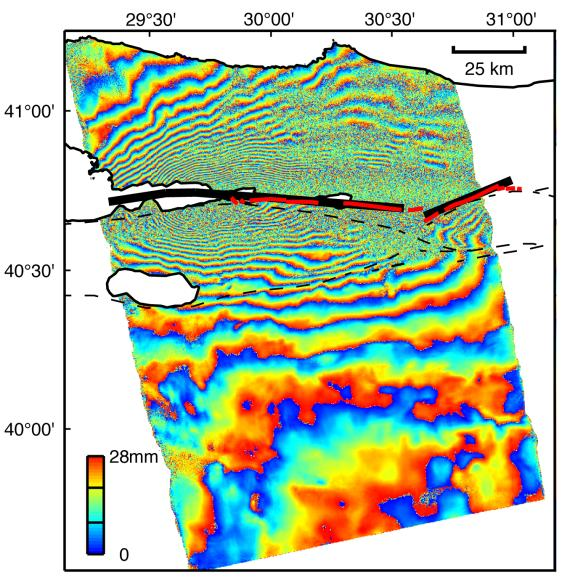
\includegraphics[height=155pt]{izmit_interferogram.jpg}
        \caption{Az izmiti (Törökország) földrengés interferogramja a becsomagolt fázissal. A földrengés előtt és után készült felvételekből előállított interferogramon a földrengés okozta LOS irányú elmozdulások láthatóak. A fekete vonalak a szeizmikus törésvonalakat jelölik. (NASA/JPL-Caltech)}
    \end{figure}
\end{frame}


%-----------------------------------------------------------------------------

\begin{frame}{Dekorreláció és fáziskicsomagolás}
    \begin{figure}
        \centering
        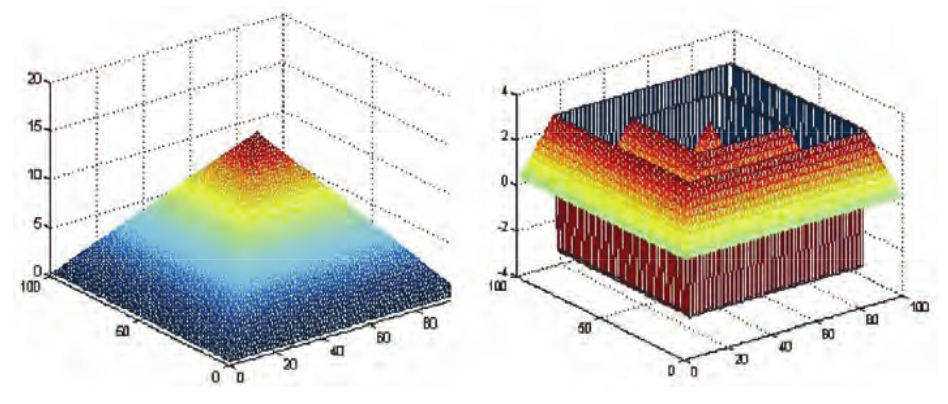
\includegraphics[width=0.6\linewidth]{esa_phase_unwrap.png}
        \caption{Fáziskicsomagolást bemutató ábra. Bal oldalon kicsomagolt-, jobb oldalon a becsomagolt fázis látható. A fáziskicsomagolás során a jobboldali ábrán látható fázisugrásokat szüntetjük meg. (InSAR Principles: Guidlines for SAR Interferomatry Processing and Iterpretation (ESA TM-19)}\label{unwrapping}
    \end{figure}
\end{frame}

%-----------------------------------------------------------------------------

\begin{frame}{A DAISY-program}
    \vspace{-10pt}
    \begin{center}
        \begin{figure}
            \begin{subfigure}[t]{.49\linewidth}
                \centering
                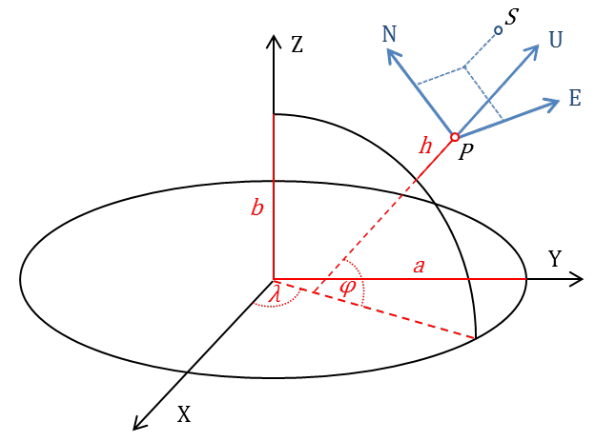
\includegraphics[height=100pt]{daisy_local_coord.png}
                \caption{Topocentrikus fel- (U), északi- (N) és keleti (E) irányok a $P$ PS-hez rögzített koordinátarendszerben. $h$ a PS pont ellipszoid feletti magassága, $\lambda$, $\phi$ a ellipszoidi koordináták, $a$ és $b$ az ellipszoid paraméterei, $S$ jelöli a műhold pozícióját.}
            \end{subfigure}
            \begin{subfigure}[t]{.49\linewidth}
                \centering
                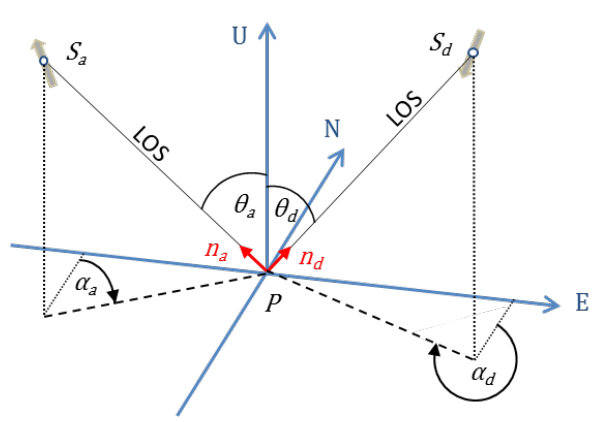
\includegraphics[height=100pt]{daisy_schematic.png}
                \caption{Felszálló és leszálló LOS irányok geometriája a lokális PS koordinátarendszerben. $S_{\text{d}}$ és $S_{\text{d}}$ a felszálló és leszálló műholdpozíciók, $\alpha_{\text{a}}$ és $\alpha_{\text{d}}$ az azimut szögek, $\theta_{\text{a}}$ és $\theta_{\text{d}}$ a beesési szögek, $n_{\text{a}}$, $n_{\text{d}}$ a felszálló és leszálló irányú LOS sebességek normálvektorjai.}
            \end{subfigure}
        \caption{A felszálló- és leszálló irányú felvételek geometriája a lokális (UNE) koordinátarendszerben.}
        \end{figure}
    \end{center}
\end{frame}

%-----------------------------------------------------------------------------

\begin{frame}{A Csomád-vulkán}
    \begin{figure}
        \centering
        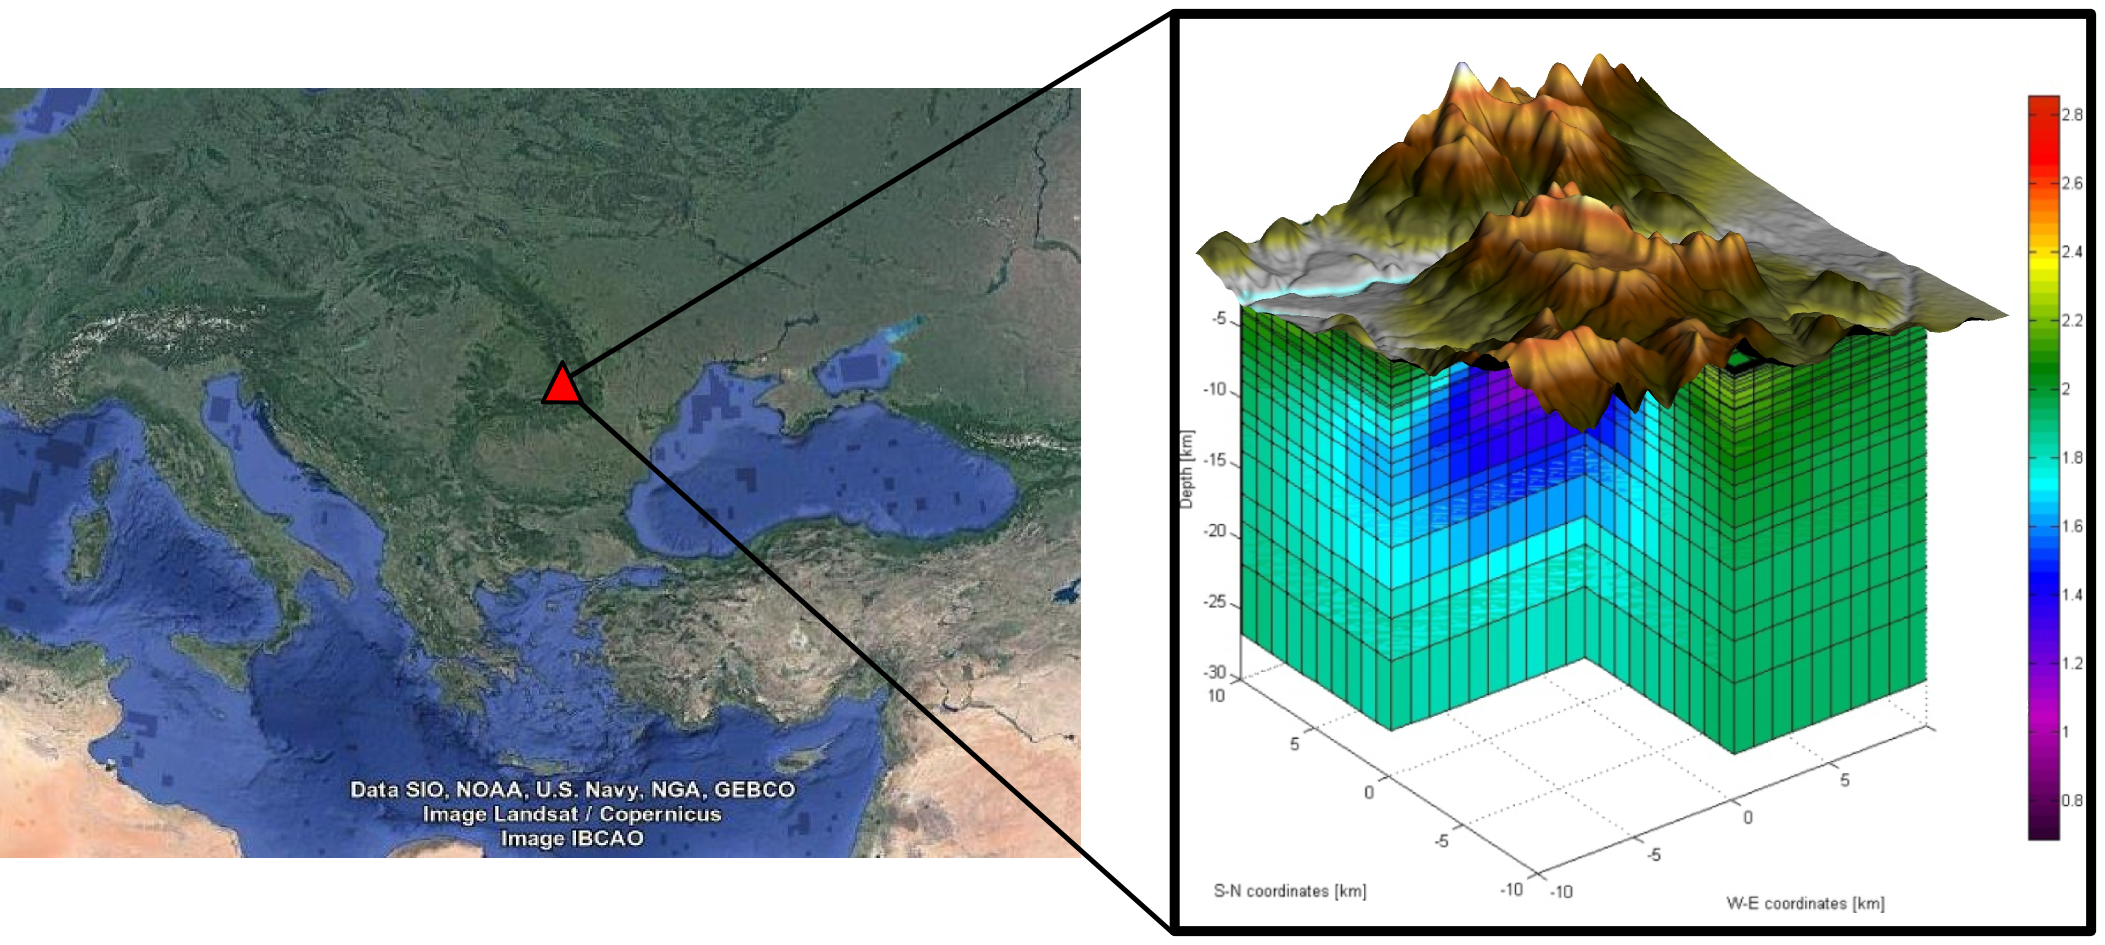
\includegraphics[height=145pt]{google_earth_csomad_harangi.png}
        \caption{A Csomád-vulkán elhelyezkedése a Kárpát-kanyar területén, a baloldali képen. Jobbra a vulkán domborzati modellje látható, alatta a magnetotellurikus mérések alapján inverzióval meghatározott fajlagos ellenállás értékek. A színskála logaritmikus, az ellenállás értékek dimenziója $\si{\ohm\meter}$}.
    \end{figure}
\end{frame}

%-----------------------------------------------------------------------------

\begin{frame}{Envisat felvételek}
    \begin{itemize}
        \item Envisat, ASAR detektor - C sáv, $\lambda = \SI{5.6}{\centi\meter}$, $f \approx \SI{5.3}{\giga\hertz}$
        \item GGI - ESA Scientific Project Proposal CAT-1 30142
        \item 23 felszálló és 32 leszálló irányú felvétel
        \item nagy térbeli és időbeli bázisvonalak $\rightarrow$ dekorreláció, inkoherens képek
    \end{itemize}

\end{frame}

%-----------------------------------------------------------------------------

\begin{frame}{SBAS interferogram hálózat}
    \begin{center}
        \begin{figure}
            \begin{subfigure}[t]{.49\linewidth}
                \centering
                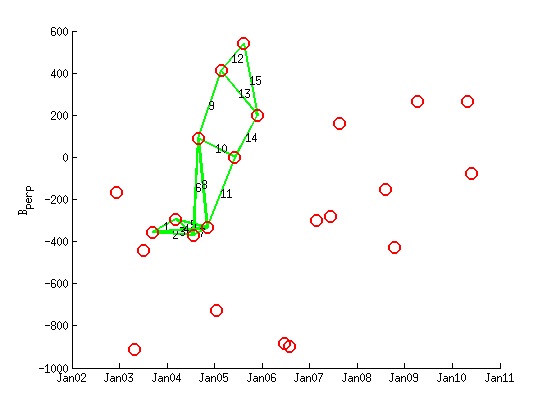
\includegraphics[height=145pt]{asc_sbas_select.png}
                \caption{Felszálló irányú felvételekből kialakított SBAS interferogram hálózat.}
            \end{subfigure}
            \begin{subfigure}[t]{.49\linewidth}
                \centering
                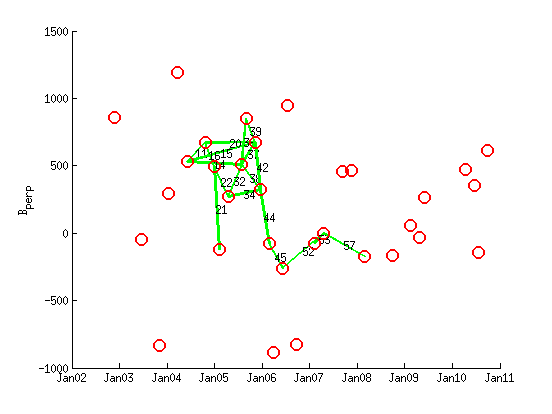
\includegraphics[height=145pt]{dsc_sbas_select.png}
                \caption{Leszálló irányú felvételekből kialakított SBAS interferogram hálózat.}
            \end{subfigure}
        \caption{SBAS hálózat leszálló- és felszálló irányú, szelektált interferogramok esetén.}
        \end{figure}
    \end{center}
\end{frame}

%-----------------------------------------------------------------------------

\begin{frame}{Felszálló és leszálló LOS sebességek}
    \begin{figure}
        \centering
        \includegraphics[height=175pt]{asc_des_los_horiz.png}
    \end{figure}
\end{frame}

%-----------------------------------------------------------------------------

\begin{frame}{DAISY Domináns Pontok}
    \begin{figure}
        \centering
        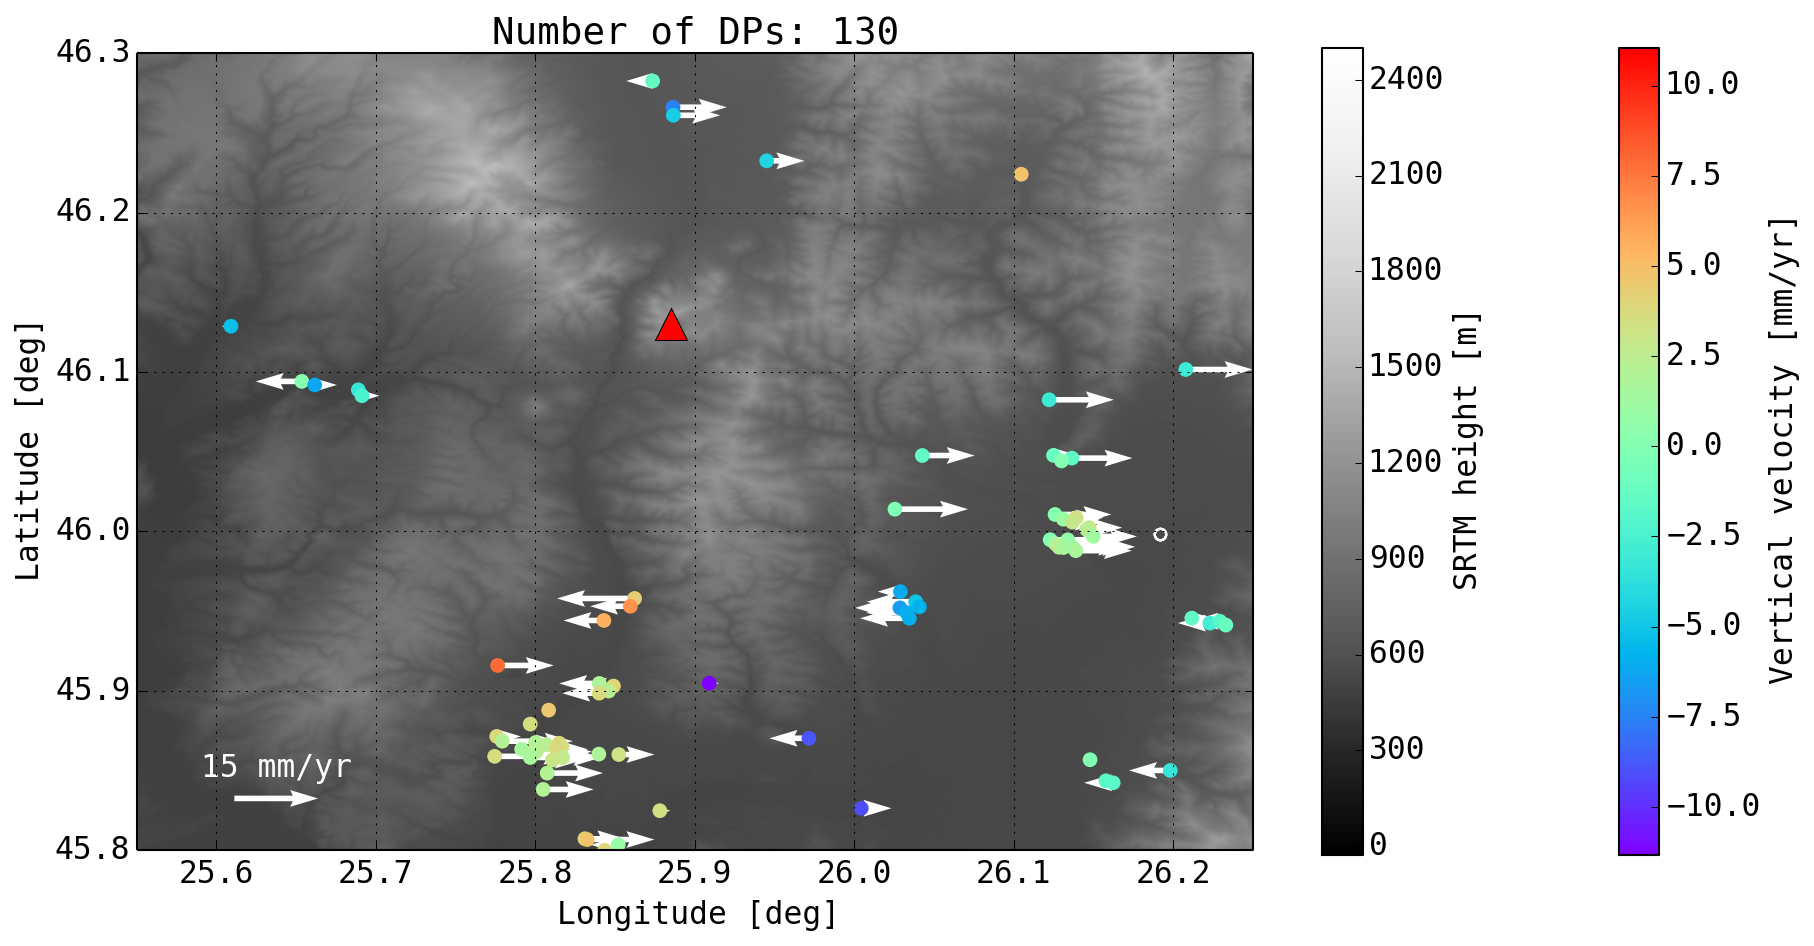
\includegraphics[height=200pt]{dp.png}
    \end{figure}
\end{frame}

%-----------------------------------------------------------------------------

\begin{frame}{Számított vertikális- és kelet-nyugati sebességkomponensek}
    \begin{figure}
        \centering
        \includegraphics[height=175pt]{grid_dp_vel.png}
    \end{figure}
\end{frame}

%-----------------------------------------------------------------------------

\begin{frame}{GNSS vs. InSAR sebességek}
    \begin{figure}
        \centering
        \includegraphics[height=200pt]{hoeven_gps_vs_insar_vert_colorbar.png}
    \end{figure}
\end{frame}

%-----------------------------------------------------------------------------

\begin{frame}{Összefoglalás}
    \begin{itemize}
        \item InSAR technológia alkalmazása Kárpát-kanyar régió, Csomád-vulkán
        \item kihívások - erős vegetáció, inkoherens interferogramok
        \item GGI által fejlesztett DAISY-program alkalmazása, vertikális és kelet-nyugati komponensek
        számítása
        \item eredmények összehasonlítása GNSS adatokkal
    \end{itemize}
\end{frame}

%-----------------------------------------------------------------------------

\begin{frame}
\center{\LARGE {\color{blue} Köszönöm a figyelmet!}\\[25pt]
Köszönet Szűcs Eszternek, Bányai Lászlónak és Wesztergom Viktornak!
}

\end{frame}

\backupbegin

%-----------------------------------------------------------------------------

\begin{frame}{Felbontási cella felületi torzulásai}
    \begin{figure}
        \centering
        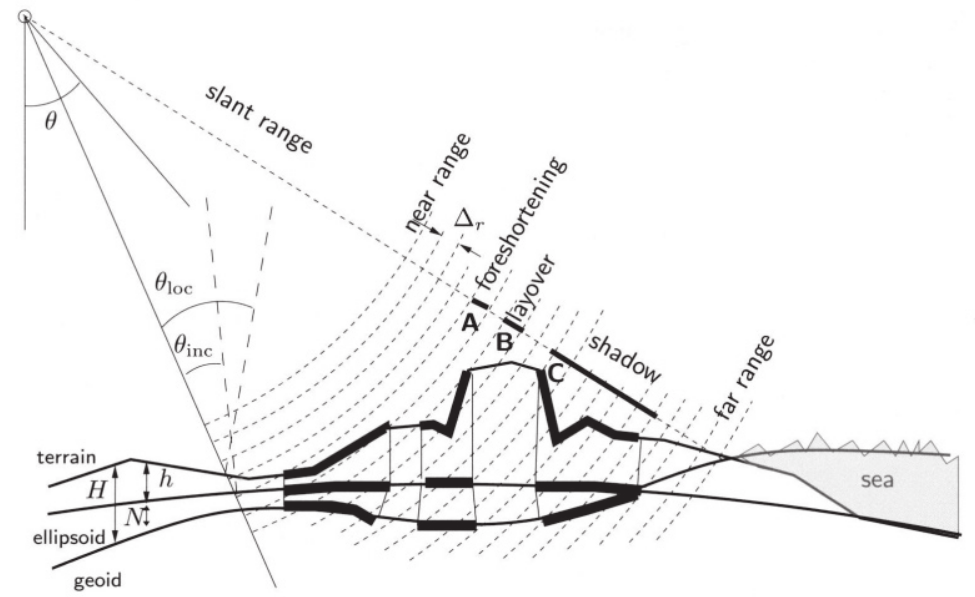
\includegraphics[height=145pt]{ramon_shortening.png}
        \caption{A felbontási cella különböző geometriai torzulásokat szenvedhet a topográfia miatt. Pl. \textit{elő-rövidülés} (foreshortening) és \textit{takarás} (layover) esetén a felbontási cellához tartozó terület nagyobb, illetve kisebb lesz. Az is előfordulhat, hogy a topográfia ``leárnyékolja'' egy, vagy több pixelhez tartozó földfelszíni felületet (\textit{shadow}).}
    \end{figure}
\end{frame}
%-----------------------------------------------------------------------------

\begin{frame}{Topográfiai fázis}
    \begin{center}
        \begin{figure}
            \centering
            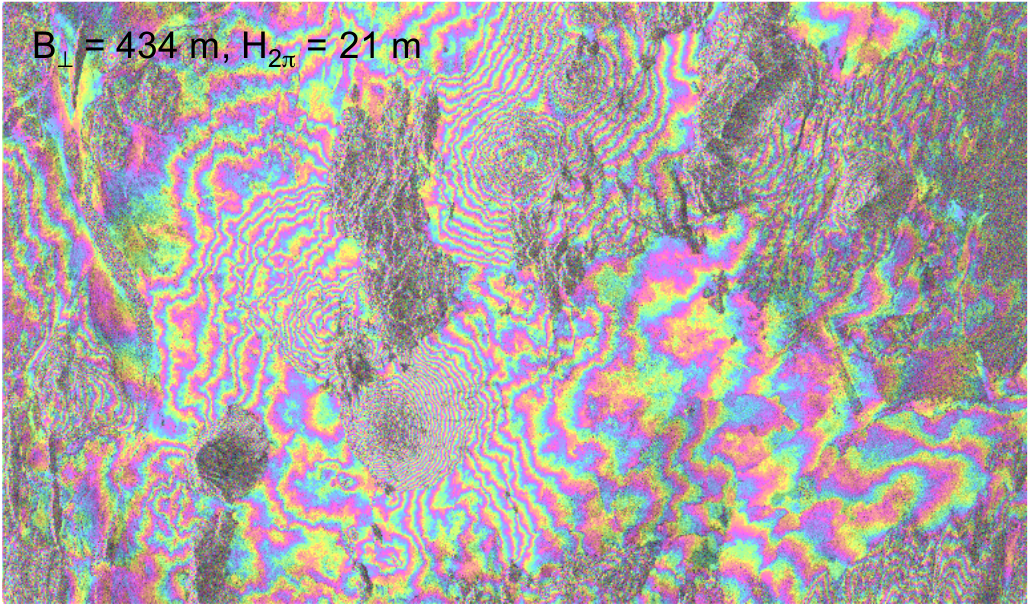
\includegraphics[height=155pt]{hooper_topo_2.png}
            \caption{Topográfiai fázist tartalmazó interferogram. Háttérben a SAR amplitudó kép látható. A színskála a becsomagolt fázisértékeket mutatja. Egy interferencia csík adott szintemelkedésnek felel meg, mely függ a merőleges bázisvonaltól.}
        \end{figure}
    \end{center}
\end{frame}

%-----------------------------------------------------------------------------

\begin{frame}{Különböző típusú szórópontok}
    \begin{figure}
        \centering
        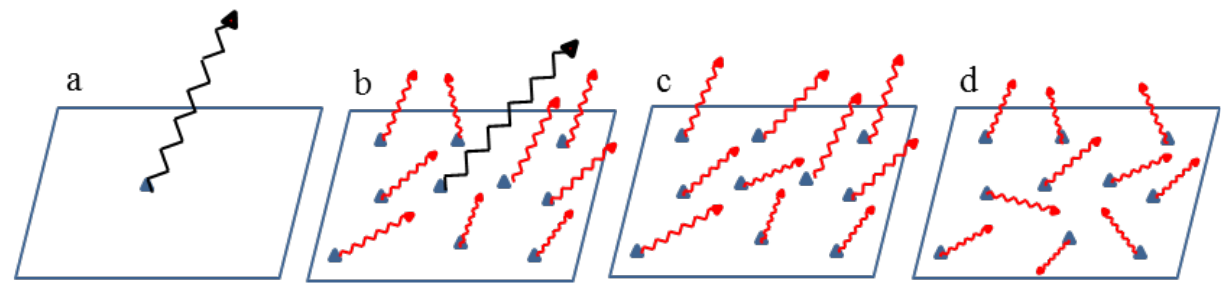
\includegraphics[height=100pt]{scatterers.png}
        \caption{Különböző szórópontokkal rendelkező pixelek: (a) egyetlen szórópontot tartalmazó pixel, (b) domináns és elosztott szórópontokat tartalmazó pixel, (c) elosztott szórópontokat tartalmazó koherens pixel, (d) elosztott szórópontokat tartalmazó inkoherens pixel.}
    \end{figure}
\end{frame}

%-----------------------------------------------------------------------------

\begin{frame}{PSI vs SBAS}
    \begin{figure}
        \centering
        \includegraphics[height=160pt]{psi_vs_sbas.png}
        \caption{PSI és SBAS interferogramok hálózata. A fekete körök jelölik a SAR felvételeket, a folytonos vonalak a két kép között készült interferogramot. $B_{\perp}$ jelöli a merőleges bázisvonal értékét.}
    \end{figure}
\end{frame}

%-----------------------------------------------------------------------------

\begin{frame}{Fázistagok tér- és időbeli jellemzői}
    \begin{table}[H]
        \centering
        \begin{tabular}{l l l} \toprule
            Fázistag & térbeli jellemző & időbeli jellemző\\ \midrule
            $\Phi_{\text{def}}$ & hosszú hullámhosszú & alacsony frekvenciájú\\
            $\Delta\Phi_{\text{DEM}}$ & hosszú hullámhosszú & bázisvonallal korrelált \\
            $\Delta\Phi_{\text{atmo}}$ & hosszú hullámhosszú & magas frekvenciájú\\
            $\Delta\Phi_{\text{pálya}}$ & hosszú hullámhosszú & magas frekvenciájú \\
            $\Phi_{\text{zaj}}$ & rövid hullámhosszú & magas frekvenciájú \\ \bottomrule
        \end{tabular}
        \caption{$\Delta\Phi$ interferometrikus fázis tagjainak tér- és időbeli jellemzői.}
    \end{table}
\end{frame}

%-----------------------------------------------------------------------------

\begin{frame}{Szeizmikus tomográfia szelvény a Kárpát-kanyar alatt}
    \begin{figure}
        \centering
        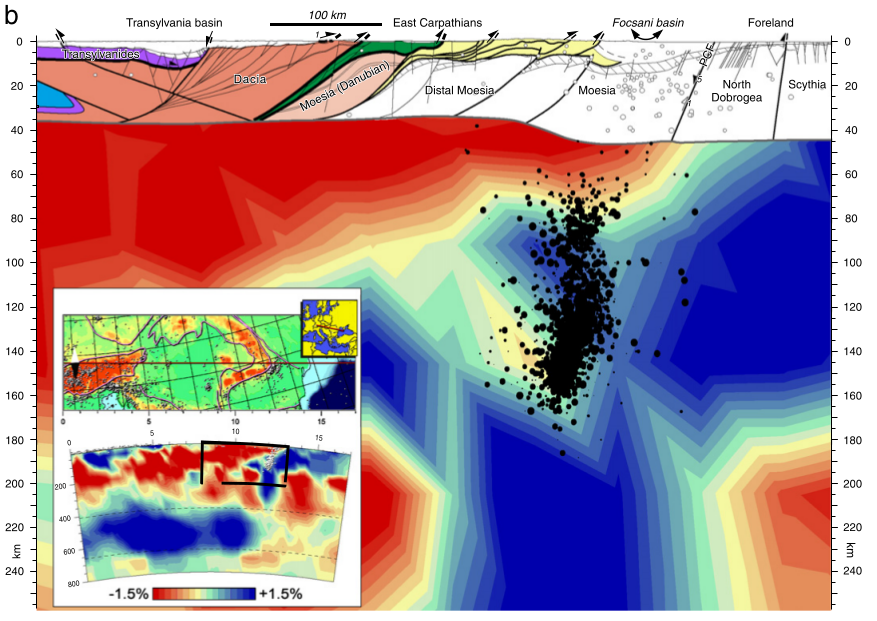
\includegraphics[height=160pt]{seism_tomo.png}
        \caption{P-hullám szeizmikus tomográfia szelvény, mely tartalmazza Kárpáti-kanyarulat régiót. A fekete pontok a kipattant földrengések hipocentrumait jelölik.}
    \end{figure}
\end{frame}

\begin{frame}{GNSS vertikális sebességek}
    \begin{center}
        \begin{figure}
            \begin{subfigure}[t]{.40\linewidth}
                \centering
                \includegraphics[height=190pt]{hoeven_gps_with_graticule.png}
            \end{subfigure}
            \begin{subfigure}[t]{.40\linewidth}
                \centering
                \includegraphics[height=195pt]{schmitt_vertical.png}
            \end{subfigure}
        \end{figure}
    \end{center}
\end{frame}

%-----------------------------------------------------------------------------

\begin{frame}{GNSS horizontális sebességek}
    \begin{center}
        \begin{figure}
            \begin{subfigure}[t]{.4\linewidth}
                \centering
                \includegraphics[height=190pt]{hoeven_horizontal.png}
            \end{subfigure}
            \begin{subfigure}[t]{.4\linewidth}
                \centering
                \includegraphics[height=195pt]{schmitt_horizontal.png}
            \end{subfigure}
        \end{figure}
    \end{center}
\end{frame}

%-----------------------------------------------------------------------------

\begin{frame}{Inkoherens és koherens interferogram}
    \begin{center}
        \begin{figure}
            \begin{subfigure}[t]{.4\linewidth}
                \centering
                \scalebox{1}[-1]{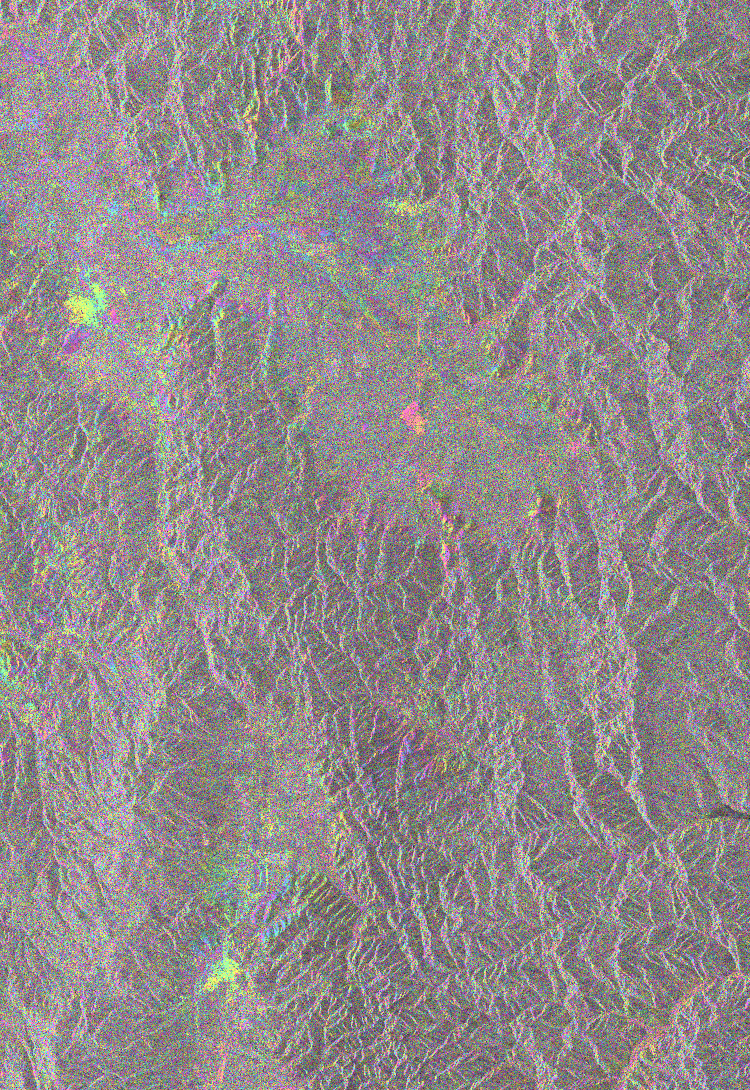
\includegraphics[height=160pt]{ifg_bad.png}}
                \caption{Inkoherens interferogram.}
            \end{subfigure}
            \begin{subfigure}[t]{.4\linewidth}
                \centering
                \scalebox{1}[-1]{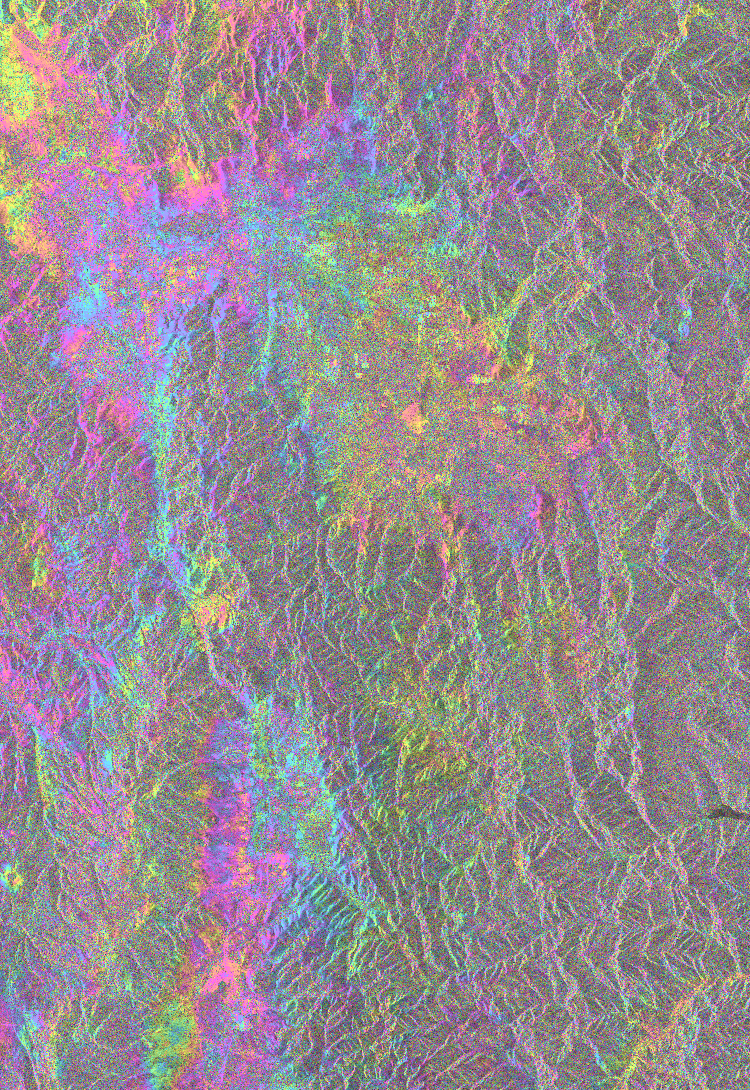
\includegraphics[height=160pt]{ifg_good.png}}
                \caption{Koherens interferogram.}
            \end{subfigure}
        \end{figure}
    \end{center}
\end{frame}

%-----------------------------------------------------------------------------

\begin{frame}{Becsomagolt fázisértékek}
    \begin{center}
        \begin{figure}
            \begin{subfigure}[t]{.49\linewidth}
                \centering
                \includegraphics[height=190pt]{asc_weed_08.png}
            \end{subfigure}
            \begin{subfigure}[t]{.49\linewidth}
                \centering
                \includegraphics[height=190pt]{asc_weed_08_zoom.png}
            \end{subfigure}
        \end{figure}
    \end{center}
\end{frame}

%-----------------------------------------------------------------------------

\begin{frame}{LOS sebességek hisztogramja}
    \begin{center}
        \begin{figure}
            \begin{subfigure}[t]{.49\linewidth}
                \centering
                \includegraphics[height=145pt]{hist_asc.png}
                \caption{Felszálló irányú felvételekből számított LOS sebességek hisztogramja.}
            \end{subfigure}
            \begin{subfigure}[t]{.49\linewidth}
                \centering
                \includegraphics[height=145pt]{hist_dsc.png}
                \caption{Leszálló irányú felvételekből számított LOS sebességek hisztogramja}
            \end{subfigure}
        \end{figure}
    \end{center}
\end{frame}

\backupend

\end{document}
